\chapter{Conclusão e Trabalhos Futuros}\label{Cap:Conclusion}

Este trabalho apresentou uma modelagem de transmissão de streaming de vídeo em 360 graus com ladrilhos que consideravam diferentes padrões de ladrilhamento em uma ampla faixa de níveis de qualidade de vídeo (isto é, taxas de bits) e propriedades SI/TI. A partir dos resultados, as distribuições Log-Normal, Gaussiana Inversa e Birnbaum-Saunders ajustaram-se melhor aos dados experimentais na maioria dos casos. Tais distribuições são muito flexíveis e interessantes para fins de modelagem matemática (por exemplo, aplicação a modelos de filas). O tempo de decodificação do ladrilho está fortemente correlacionado com a taxa de bits do ladrilhos somente se a qualidade do vídeo for alta, e o grau de correlação diminui se o número de ladrilhos por quadro aumentar (ou seja, alta segmentação do bloco). O padrão de ladrilho $6 \times 3$ proporcionou o melhor equilíbrio entre o tempo de decodificação e a taxa de bits média, ao mesmo tempo que apresentou boas propriedades de correlação entre ambas as métricas se altos níveis de qualidade forem usados. Tal informação pode possivelmente ser usada por algoritmos ABR baseados em DASH para inferir o tempo de decodificação dos ladrilhos.

Como trabalho futuro planejamos projetar um algoritmo de adaptação de qualidade utilizando as métricas de desempenho analisadas e então avaliá-lo em um ambiente virtual de simulação de rede usando o simulador NS-3\footnote{https://www.nsnam.org/} conectado a servidores locais reais rodando em containers Docker. Considerando o registro de movimento de cabeça e que todos os segmentos acessados pelo cliente serão sempre os mesmos para cada usuário, será possível avaliar diferentes tipos de algoritmos sob diferentes infraestruturas sob as mesmas condições de usuário. Então, usando o modelo de qualidade desenvolvido neste trabalho será possível avaliar de forma objetiva a capacidade dos algoritmos se adaptarem às condições de rede em um ambiente bem controlado, como o mostra a figura~\ref{fig:modelo_simulação}.

\begin{figure}[h]
    \centering
    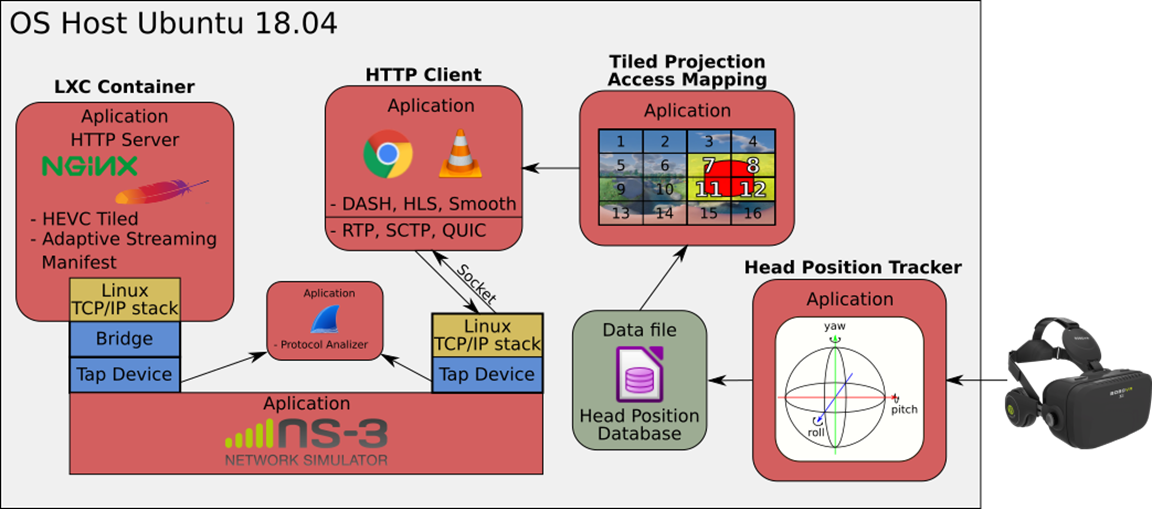
\includegraphics[width=0.8\linewidth]{fig/modelo_simulação.png}
    \caption{Modelo de simulação que será usado para avaliação}
    \label{fig:modelo_simulação}
\end{figure}


\section{Trabalhos futuros}

\section{Cronograma}


